\documentclass[a4paper, 10pt, twocolumn, twoside]{book}

\usepackage{fontspec}
\setmainfont{Sublimation Medium}

\usepackage{pgf}
\usepackage{tikz}
\usetikzlibrary{fadings}
\usetikzlibrary{patterns}
\usetikzlibrary{external}
\usetikzlibrary{calc}
\usepackage{xcolor}
\definecolor{steelblue}{HTML}{B0C4DE}
%\tikzexternalize[prefix=figures/]

\usepackage{geometry}
  \geometry{a4paper, 
  includeheadfoot,
  top=0cm, 
  headheight=23mm, 
  headsep=7mm, 
  footskip=23mm, 
  bottom=7mm,
  left=20mm, 
  right=15mm
  }  
  
\graphicspath{{./SR5_Fankit/}}
  

  
\begin{document}
%\tikzsetfigurename{cover}
\begin{tikzpicture}[remember picture, overlay, shift={(current page.center)}]

\tikzstyle{reverseclip}=[insert path={(current page.north east) --
  (current page.south east) --
  (current page.south west) --
  (current page.north west) --
  (current page.north east)}
]

\makeatletter
\tikzset{use path/.code=\tikz@addmode{\pgfsyssoftpath@setcurrentpath#1}}
\makeatother

\coordinate (TL) at ({(-.5\paperwidth)+20mm}, 9.5cm);
\coordinate (BL) at ({(-.5\paperwidth)+20mm},{(-.5\paperheight)+23mm});
\coordinate (BR) at (.5\paperwidth-20mm,{(-.5\paperheight)+23mm});
\coordinate (TR) at (.5\paperwidth-20mm, 9.5cm);

\path [save path=\outline] (TL) -- ++(0,-3cm) -- ++(-45:5mm) -- ++(0,-8cm) -- ++(-135:5mm) -- ($(BL)+(0, 5mm)$) -- ($(BL)+(5mm, 0)$) -- (0,{(-.5\paperheight)+20mm}) -- ++(45:5mm) -- ($(BR)+(-3mm,3.54mm)$) -- ($(BR)+(0,5.54mm)$) -- (TR) -- cycle;

\begin{scope}
\begin{pgfinterruptboundingbox}
\path [clip] (TL) -- ++(0,-3.5cm) -- ++(-45:5mm) -- ++(0,-8.5cm) -- ++(-135:5mm) -- ($(BL)+(0, 5mm)$) -- ($(BL)+(5mm, 0)$) -- (0,{(-.5\paperheight)+23mm}) -- ++(45:5mm) -- ($(BR)+(-6mm,3.54mm)$) -- ($(BR)+(-3mm,6.54mm)$) -- ++(0,3.2cm) -- ++(45:4.24264mm) -- ++(0, 4cm) -- ++(120:6mm) -- ++(0,10.5cm) -- ++(60:6mm) -- (TR) -- cycle [reverseclip];
\end{pgfinterruptboundingbox}
\node at (-.5\paperwidth,0) {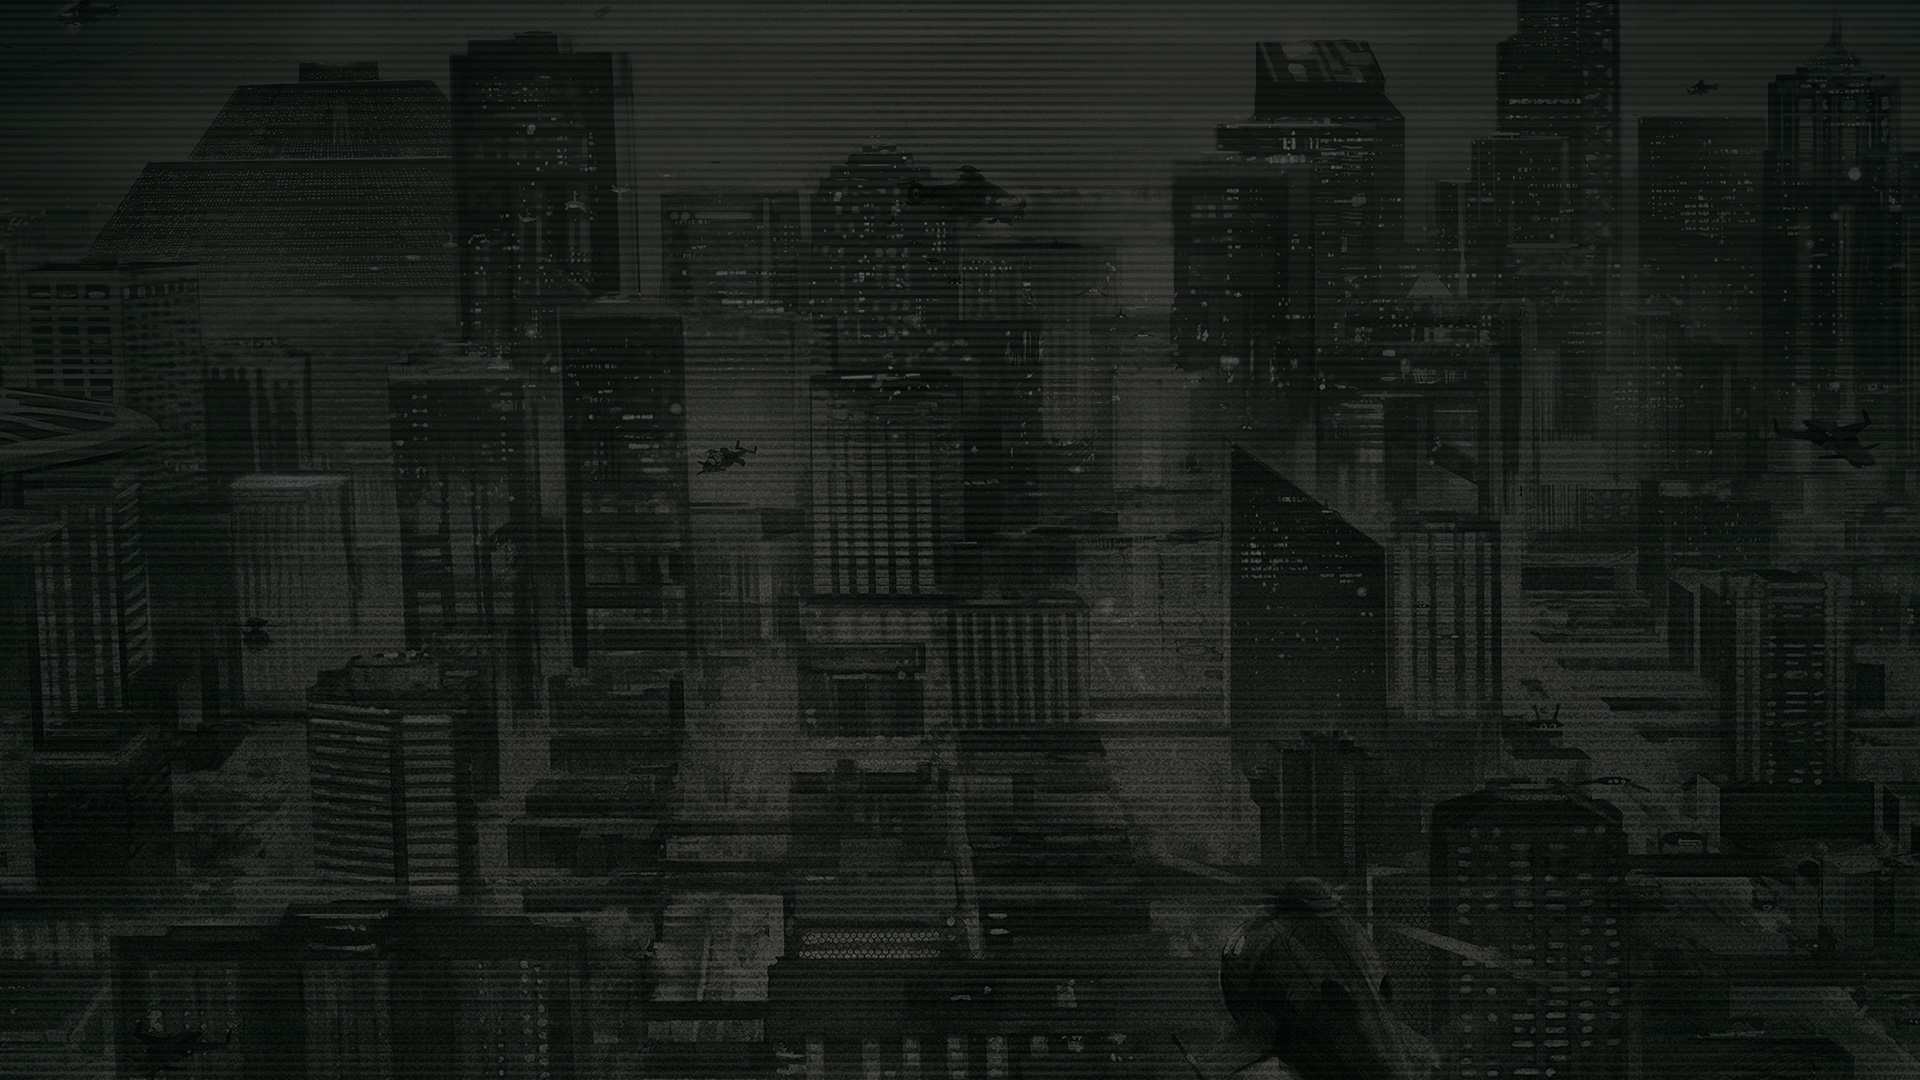
\includegraphics[width=2\paperwidth, height=\paperheight]{Hintergruende/Skyline_Seattle_schwarz_1920x1080px.jpg}};
\node[opacity=.25] at (-.5\paperwidth,0) {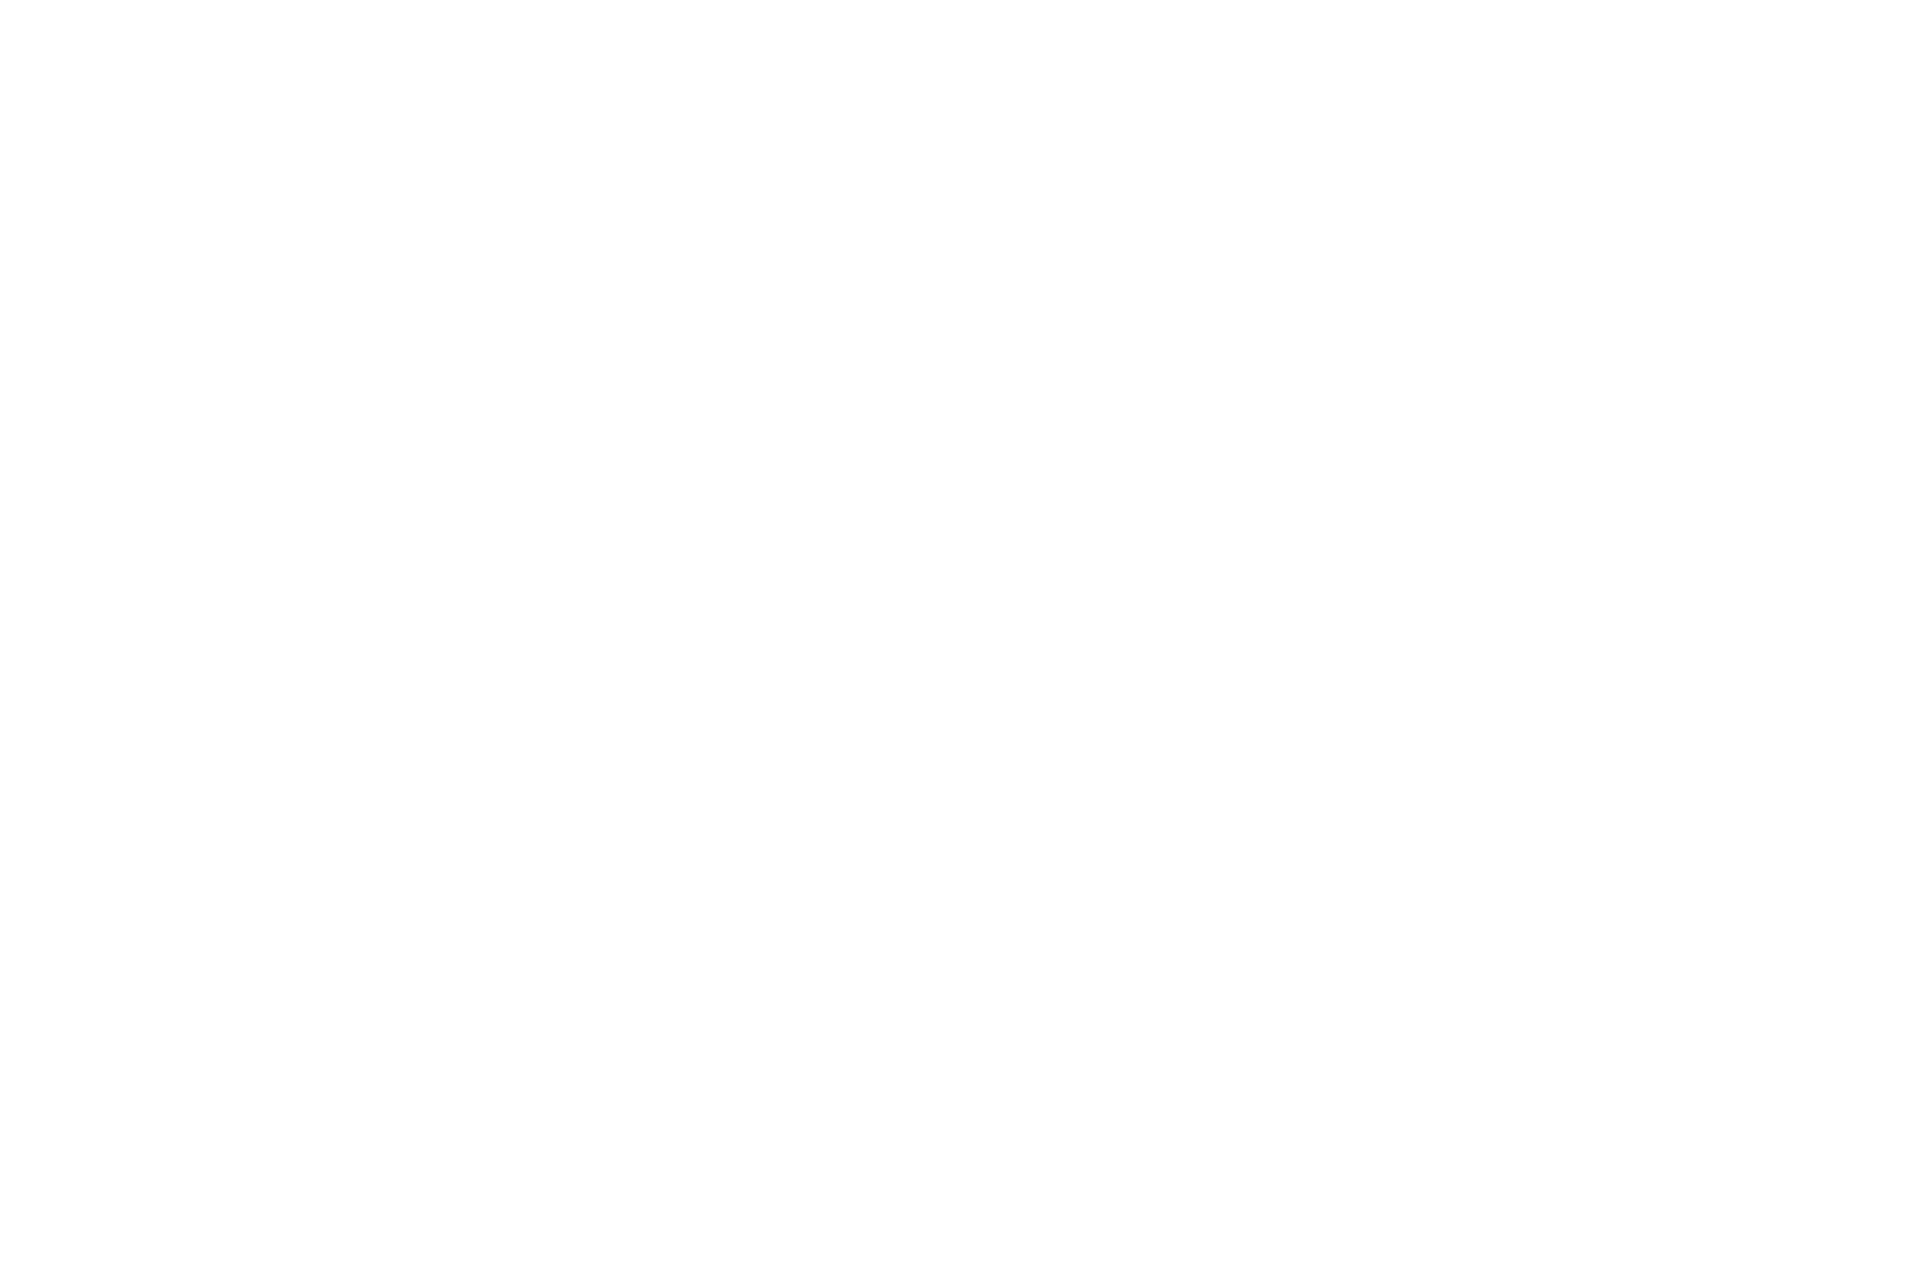
\includegraphics[width=2\paperwidth, height=1.1\paperheight]{Hintergruende/Interface_1920x1280px.png}};
\fill[brown, opacity=.2] (-.5\paperwidth, -.5\paperheight) rectangle (.5\paperwidth, .5\paperheight);
\path[draw, line width=4mm, color=steelblue, opacity=.75](TL) -- ++(0,-3.5cm) -- ++(-45:5mm) -- ++(0,-8.5cm) -- ++(-135:5mm) -- ($(BL)+(0, 5mm)$) -- ($(BL)+(5mm, 0)$) -- (0,{(-.5\paperheight)+23mm}) -- ++(45:5mm) -- ($(BR)+(-6mm,3.54mm)$) -- ($(BR)+(-3mm,6.54mm)$) -- ++(0,3.2cm) -- ++(45:4.24264mm) -- ++(0, 4cm) -- ++(120:6mm) -- ++(0,10.5cm) -- ++(60:6mm) -- (TR) -- cycle;
\path[draw, line width=1mm, color=black, opacity=.5](TL) -- ++(0,-3.5cm) -- ++(-45:5mm) -- ++(0,-8.5cm) -- ++(-135:5mm) -- ($(BL)+(0, 5mm)$) -- ($(BL)+(5mm, 0)$) -- (0,{(-.5\paperheight)+23mm}) -- ++(45:5mm) -- ($(BR)+(-6mm,3.54mm)$) -- ($(BR)+(-3mm,6.54mm)$) -- ++(0,3.2cm) -- ++(45:4.24264mm) -- ++(0, 4cm) -- ++(120:6mm) -- ++(0,10.5cm) -- ++(60:6mm) -- (TR) -- cycle;
\end{scope}
\node at (0,11cm) {
\includegraphics[scale=.4]{Logo/Shadowrun-5-Logo_1500x600px.png}};
\node[anchor=north east, align=right, white, font=\bfseries\Large] at ($(BR)+(-6.2mm,0.2mm)$) {HOMEBREW BOOK};
\node[anchor=north east, align=right, steelblue, font=\bfseries\Large, opacity=.7] at ($(BR)+(-6mm,0)$) {HOMEBREW BOOK};
\end{tikzpicture}
%\tikzsetfigurename{footerleft}
%\begin{tikzpicture}


%\end{tikzpicture}
%\tikzsetfigurename{footerright}
%\begin{tikzpicture}


%\end{tikzpicture}

\end{document}